\documentclass[a4paper, 11pt]{article}
%\documentclass[pre,amsmath,aps,superscriptaddress,a4paper]{revtex4}
\usepackage{graphicx,xspace,units,subfigure}
\usepackage{float}
\usepackage{amsmath}
\usepackage{amssymb}
\usepackage[normalem]{ulem}
\usepackage{appendix}
\usepackage{hyperref}
\usepackage{setspace}
%\usepackage{helvet}
\usepackage{wrapfig}
\usepackage{eurosym}
%\usepackage{xcolor}
\usepackage{multirow}
\usepackage[dvipsnames]{xcolor}
\usepackage{comment}

% make a header
\usepackage{fancyhdr}
\pagestyle{fancy}
%\rhead{this is page \thepage}
%\chead{center of the footer!}
\renewcommand{\headrulewidth}{0.4pt}
%\renewcommand{\footrulewidth}{0.4pt}
\newlength\FHoffset
\setlength\FHoffset{0.1cm}
\addtolength\headwidth{2\FHoffset}
\fancyheadoffset{\FHoffset}

% Use sans serif throughout 
%\usepackage{fontspec}
%\renewcommand{\familydefault}{\sfdefault}
%\setsansfont{Helvetica}
  
\singlespacing
%\onehalfspacing
%\doublespacing
%\setstretch{1.1}

\usepackage{cite}          % writes reference [1,2,3] --> [1-3]
\usepackage{sectsty}     % center section without centering the subsections...
\sectionfont{\centering} % center section without centering the subsections...
\usepackage[font=small,labelfont=bf]{caption} % caption font size

%% Language and font encodings
\usepackage[english]{babel}
%\usepackage[utf8x]{inputenc}
%\usepackage[T1]{fontenc}

%% Sets page size and margins
\usepackage[a4paper,top=1.5cm,bottom=1.5cm,left=2cm,right=2cm]{geometry}
%\usepackage[a4paper,top=1.5cm,bottom=1.5cm,left=2cm,right=2cm,marginparwidth=1.75cm]{geometry}

\usepackage{color}
%\usepackage{helvet}
%\fontfamily{phv}
\usepackage{mdframed}

\newcommand{\be}{\begin{equation}}
\newcommand{\ee}{\end{equation}}

% \documentclass[a4paper, 11pt]{article}
% \usepackage[utf8]{inputenc}
% \usepackage{helvet}
% \fontfamily{phv}


% \usepackage{fullpage} % changes the margin





\begin{document}
\section*{Implementation of elasticity in sensory-growth rod-like organs}
\subsection*{Introduction}
This paper describes how to combine our formalism of active reorientations of growing rods with M. Gazzola's Cosserat filament integrator (see \emph{Gazzola RSOS 2018}). To do so, we separate growth and elasticity, following the mathematical formalism presented in A. Goriely's book (\emph{The Mathematics and Mechanics of Biological Growth, Springer 2017}). The mathematical decomposition of growth and elastisity originates from a distinct separation of timescales: the timescale of growth processes in plants is in the order of $10^4$ seconds, while their elastic relaxation times are of the order of $1-0.01$ seconds. We can therefore assume that the dynamics of a growing plant are in the quasi-static regime, in which the organ reaches its mechanical steady state for every growth step.

\begin{figure}[h!]
    \centering
    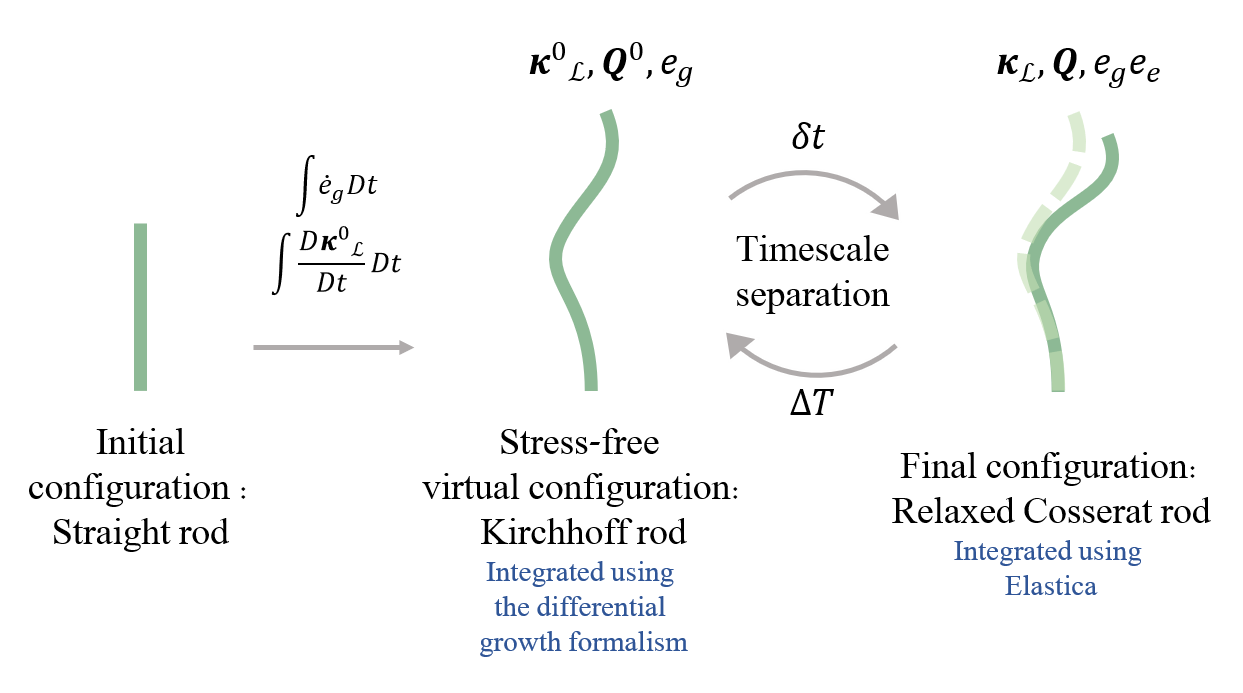
\includegraphics[width=0.80\textwidth]{growth_concept.png}
    \caption{\textbf{Integration scheme}. Strating from a straight rod, growth is implemented by updating the rest lengths and rest curvature vectors of the Cosserat rod according to the active growth model. One can think of rest lengths and curvatures as describing a referential stress-free virtual rod, as described in Goriely's book. Then, the Cosserat rod relaxes into its new stable mechanical state using Elatsica. The active growth step and passive mechnanical relaxation is iterated, and only the final relaxed configurations are collected.} \label{fig:fig1}
\end{figure}

Practically, we start from a straight rod clamped on one side, and let it grow.Growth is implemented by updating the rest lengths and rest curvature vectors of the Cosserat rod according to the active growth model. One can think of rest lengths and curvatures as describing a referential stress-free virtual rod, as described in Goriely's book. Then, the Cosserat rod relaxes into its new stable mechanical state using Elatsica. The active growth step and passive mechnanical relaxation is iterated, and only the relaxed configurations of each growth step are collected.\\
To execute this integration scheme, new basic function must be introducted to the Cosserat rod class in Elastica:
\begin{itemize}
    \item \underline{Set growth parameters}: Defines the growth profile of the organ, including its growth zone and groath rate profile. Should be defined once before integration.
    \item \underline{Define tropisms}: Defines the active mechanisms that govern the dynamics of the rest curvture, based on our tropism model. Should be defined once before integration.
    \item \underline{Update growth}: Preforms a growth timestep: Updates the rest lengths and rest curvatures according to the given active growth mechanisms.
    \begin{itemize}
        \item \underline{Divide elements:} If an element grew above a given rest length threshold it is divided into two "daughter" elements. 
    \end{itemize}
   
\end{itemize} 
We now go over each function in detail. 

\subsection*{Update growth}
The basic principle is to decompose the total stretch in the organ into growth stretch ($e_g$) and an elastic stretch ($e_e$):
\begin{equation}
    e=e_e\cdot e_g
\end{equation}
Referring to the re-scaling of segment properties in Gazzola's 2018 paper, the growth stretch $e_g$ does not change the area or curvature of the segment, and adds mass to the segment. Therefore, the following relations hold:
\begin{equation}
    ds=e\cdot d\hat{s}=e_e\cdot e_gd\hat{s}\;,\;
    R=\frac{\hat{R}}{\sqrt{e_e}}\;,\;
    A=\frac{\hat{A}}{e_e}\;,\;
    I=\frac{\hat{I}}{e_e^2}\;,\;
    B=\frac{\hat{B}}{e_e^2}\;,\;
    S=\frac{\hat{S}}{e_e}\;,\;
    \kappa_{\mathcal{L}}=\frac{\hat{\boldsymbol{\kappa}}_{\mathcal{L}}}{e_e}
\end{equation}
The mass of the segment will be:
\begin{equation}
    dm=\rho \pi R^2 ds=e_g\rho\pi\hat{R}^2 d\hat{s}
\end{equation}
\\
\noindent \underline{Quasi-static integration:} There a distinct separation of timescales in our problem: the timescale of growth processes in plants is in the order of $10^4$ seconds, while their elastic relaxation times are of the order of $1-0.01$ seconds. We can therefore assume that the dynamics of a growing plant are in the quasi-static regime, in which the organ has reaches the steady state for every step of growth. One can thus choose to implement growth either by growing the plant in time-steps which are dictated by the elastic relaxation process (that is, growth takes place when the energy minimizes to a certain minimal threshold), or continuously growing the organ at a very slow rate. \\

\noindent \underline{Body forces ramp:} The code should run smoothly and simulate quasi static growth after an initial relaxation to external forces. Since the initial state of the organ is assumed to be a straight rod, the initial relaxation to gravity may take a while due to oscillations and their damping by dissipation. This relaxation initialization can be reduced by adding the external forces in a quasi-static manner.\\

\noindent \underline{Segment division:} For a constant profile of growth rates along the organ, after long periods of time the growth stretch $e_g$ will inevitably reach high values (for example around the apex), for which the discrete segments approximation is no longer be valid. Therefore, a "segment division" should be implemented above a certain threshold of local growth stretch $e_g$. In this division, the segment is to be split in half, while both halves should retain all of its properties but its length:
\begin{equation}
    ds_i=ds_{i,1}+ds_{i,2}
\end{equation}
The propagation of the local coordinates should be updated accordingly.
\\

\noindent \underline{Current plan:} write a code (and a wrapper?) that: 
\begin{itemize}
    \item Implements various growth rate functions $\dot{e}_g(s,t)$ (exponential, apical flat and apical Gaussian). 
    \item Limits growth time-step by maximal growth velocity (apical velocity): $v_{\text{max}}=\int_0^{L(t)}\dot{e}_g(s,t)ds$ 
    \item Divides segments that elongate over a certain threshold ($d\hat{s}>ds_{\text{max}}$). This includes the calculation of the local coordinate system (Q) of the two parts of the divided segments, and will probably require recalculations of the Voronoi regions.
    \item Propagates intrinsic curvature (and twist) according to the active growth model.
\end{itemize}



\newpage

\subsection*{Element division}
In a growing rod, if an element (or an edge) grows above a certain threshold, we need to divide it into two distinct elements. Using the code of Gazzola's lab, the division can be implemented by breaking down the element, $\boldsymbol{\ell}_i=\boldsymbol{r}_{i+1}-\boldsymbol{r}_{i}$, into two new elements (see Fig.~\ref{fig:fig1}):
\begin{equation}
    \boldsymbol{\ell}_i=\boldsymbol{\ell}_{i,1}+\boldsymbol{\ell}_{i,2}
\end{equation}


\begin{figure}[h!]
    \centering
    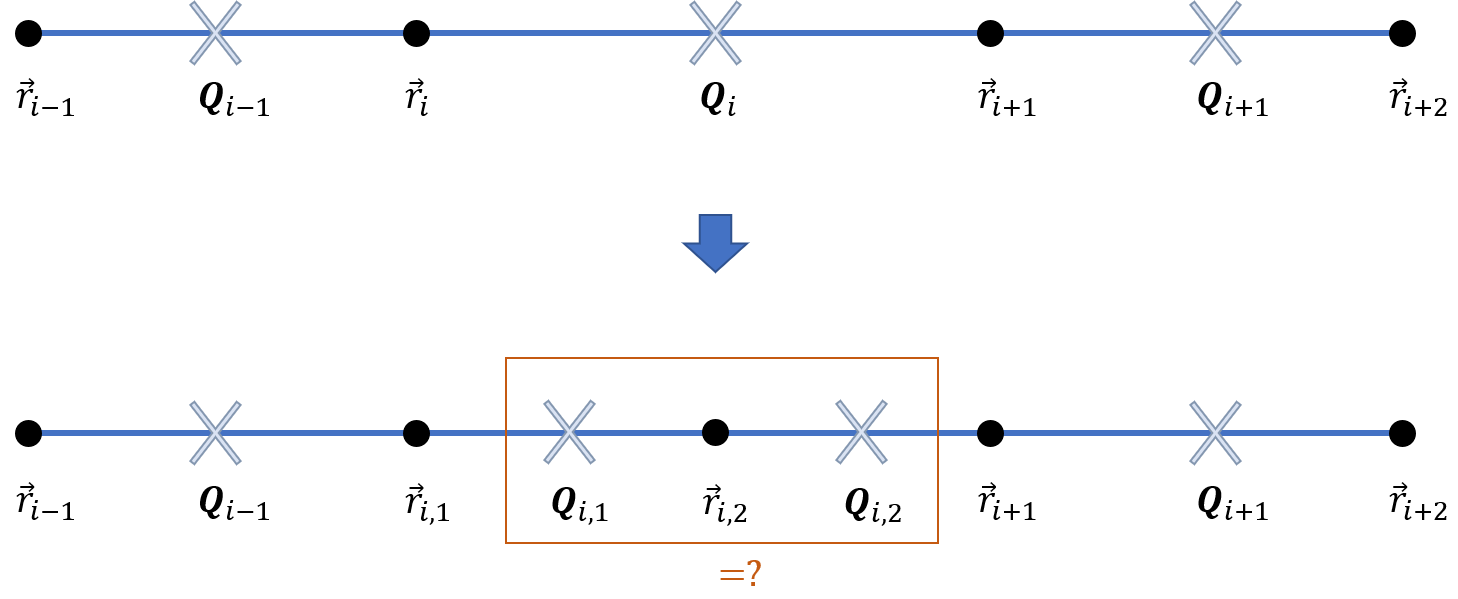
\includegraphics[width=0.80\textwidth]{seg_div.png}
    \caption{\textbf{Segment division}. One must demand continuity in $\boldsymbol{r}$, $\boldsymbol{Q}$ and $\boldsymbol{a}$ in order to find the corrects values for the characteristics of the new "daughter" elements. } \label{fig:fig1}
\end{figure}
\noindent Each segment has a variety of local variables, that are defined either pointwise on the vertices, for example the segments physical location $\vec{r}_i$ and mass $m_i$, as an edge property, such as the tangent vector $\boldsymbol{t}$ or strain $\hat{\boldsymbol{\sigma}}^i_{\mathcal{L}}$, or on the interior vertex, for example the inextensible curvature $\hat{\boldsymbol{\kappa}}_\mathcal{L}$. 
\noindent For simplicity, we assume that the rest length of the segment splits to two equal lengths, or:
\begin{equation}
\hat{\ell}_{i,1}=\hat{\ell}_{i,1}=\frac{1}{2}\hat{\ell}_i    
\end{equation}
and that the elastic stretch $e_i$ and the shear vector $\vec{\sigma}_i$ remain constant on the two "daughter" segments:
\begin{equation}
    e_{i,1}=e_{i,2}=e_{i}\;\;\;,\;\;\; \boldsymbol{\sigma}^{i,1}_\mathcal{L}=\boldsymbol{\sigma}^{i,2}_\mathcal{L}=\boldsymbol{\sigma}^i_\mathcal{L}
\end{equation}
To properly find the curvatures and the local material frames of the new segments, one must demand that the surrounding quantities remain constant, that is, that $\boldsymbol{r}_{i+1}$ and $\boldsymbol{r}_{i}=\boldsymbol{r}_{i,1}$ don't change, and neither do $\boldsymbol{Q}_{i-1}$ and $\boldsymbol{Q}_{i+1}$.\\
We start the condition on the local coordinate frames. We notice that one can write the relation between $\boldsymbol{Q}_{i-1}$ and $\boldsymbol{Q}_{i+1}$ using the Rodrigues formula twice \textcolor{blue}{(notice that it's not the same formula in the article, a minus needs to be added)}:
\begin{equation}\label{eq:Q1}
    \boldsymbol{Q}_{i+1}=\exp\left(-{\hat{\mathcal{D}}_i\hat{\boldsymbol{\kappa}}^i_\mathcal{L}}\right)\boldsymbol{Q}_i=\exp\left(-{\hat{\mathcal{D}}_i\hat{\boldsymbol{\kappa}}^i_\mathcal{L}}\right)\exp\left(-\hat{\mathcal{D}}_{i-1}\hat{\boldsymbol{\kappa}}^{i-1}_\mathcal{L}\right)\boldsymbol{Q}_{i-1}
\end{equation}
Where:
\begin{equation}
    \hat{\mathcal{D}}_i=\frac{1}{2}(\hat{\ell}_{i+1}+\hat{\ell}_{i})
\end{equation}
In a similar manner, after the division we have:
\begin{equation}\label{eq:Q2}
    \boldsymbol{Q}_{i+1}=\exp\left(-\hat{\mathcal{D}}_{i,2}\hat{\boldsymbol{\kappa}}^{i,2}_\mathcal{L}\right)\exp\left(-\hat{\mathcal{D}}_{i,1}\hat{\boldsymbol{\kappa}}^{i,1}_\mathcal{L}\right)\exp\left(-\hat{\mathcal{D}}'_{i-1}\hat{\boldsymbol{\kappa}}^{i-1}_\mathcal{L}\right)\boldsymbol{Q}_{i-1}
\end{equation}
where we notice that:
\begin{equation}
    \hat{\mathcal{D}}_{i-1}=\frac{1}{2}(\hat{\ell}_{i}+\hat{\ell}_{i-1})\neq\hat{\mathcal{D}}'_{i-1}=\frac{1}{2}(\hat{\ell}_{i,1}+\hat{\ell}_{i-1})=\frac{1}{2}(\frac{1}{2}\hat{\ell}_{i}+\hat{\ell}_{i-1})
\end{equation}
Eq.~\ref{eq:Q1} and Eq.~\ref{eq:Q2} give the continuity condition on the local coordinate frame:
\begin{equation}
    \exp\left(-{\hat{\mathcal{D}}_i\hat{\boldsymbol{\kappa}}^i_\mathcal{L}}\right)\exp\left(-\hat{\mathcal{D}}_{i-1}\hat{\boldsymbol{\kappa}}^{i-1}_\mathcal{L}\right)=\exp\left(-\hat{\mathcal{D}}_{i,2}\hat{\boldsymbol{\kappa}}^{i,2}_\mathcal{L}\right)\exp\left(-\hat{\mathcal{D}}_{i,1}\hat{\boldsymbol{\kappa}}^{i,1}_\mathcal{L}\right)\exp\left(-\hat{\mathcal{D}}'_{i-1}\hat{\boldsymbol{\kappa}}^{i-1}_\mathcal{L}\right)
\end{equation}
or explicitly:
\begin{align}\label{eq:Q_f}
    \exp\left(-{\frac{1}{2}(\hat{\ell}_{i+1}+\hat{\ell}_{i})\hat{\boldsymbol{\kappa}}^i_\mathcal{L}}\right)\exp\left(-\frac{1}{2}(\hat{\ell}_{i}+\hat{\ell}_{i-1})\hat{\boldsymbol{\kappa}}^{i-1}_\mathcal{L}\right)&=\nonumber\\
    =\exp\left(-\frac{1}{2}(\hat{\ell}_{i+1}+\frac{1}{2}\hat{\ell}_{i})\hat{\boldsymbol{\kappa}}^{i,2}_\mathcal{L}\right)&\exp\left(-\frac{1}{2}\hat{\ell}_i\hat{\boldsymbol{\kappa}}^{i,1}_\mathcal{L}\right)\exp\left(-\frac{1}{2}(\frac{1}{2}\hat{\ell}_{i}+\hat{\ell}_{i-1})\hat{\boldsymbol{\kappa}}^{i-1}_\mathcal{L}\right)
\end{align}
We can see from Eq.~\ref{eq:Q_f} that we have 2 unknowns: $\hat{\boldsymbol{\kappa}}^{i,1}_\mathcal{L}$ and $\hat{\boldsymbol{\kappa}}^{i,2}_\mathcal{L}$. To find them, we now add the requirement that the spatial vectors $\boldsymbol{r}_{i+1} $ and $\boldsymbol{r}_{i}=\boldsymbol{r}_{i,1}$ remain unchanged. To do so, we look at the expression for the strain vector:
\begin{equation}
    \boldsymbol{\sigma}^i_\mathcal{L}=\boldsymbol{Q}_i\left(\frac{\partial \boldsymbol{r}_i}{\partial \hat{s}}-\boldsymbol{d}^i_3\right)
\end{equation}
Multiplying from the left by $\boldsymbol{Q}^T_i$ and integrating by $\hat{s}$ give:
\begin{equation}\label{eq:r_1}
    \boldsymbol{r}_{i+1}=\left(\boldsymbol{Q}^T_i\boldsymbol{\sigma}^i_\mathcal{L}+\boldsymbol{d}^i_3\right)\hat{\ell}_i+\boldsymbol{r}_{i}
\end{equation}
Or:
\begin{equation}
    \boldsymbol{\ell}_i=\left(\boldsymbol{Q}^T_i\boldsymbol{\sigma}^i_\mathcal{L}+\boldsymbol{d}^i_3\right)\hat{\ell}_i
\end{equation}
In a similar fashion, we can now write the relation between $\boldsymbol{r}_{i+1} $ and $\boldsymbol{r}_{i}=\boldsymbol{r}_{i,1}$ after the division:
\begin{align}
    \boldsymbol{r}_{i+1}&=\boldsymbol{\ell}_{i,2}+\boldsymbol{\ell}_{i,1}+\boldsymbol{r}_{i}\nonumber\\
    &=\left(\boldsymbol{Q}^T_{i,2}\boldsymbol{\sigma}^{i,2}_\mathcal{L}+\boldsymbol{d}^{i,2}_3\right)\hat{\ell}_{i,2}+\left(\boldsymbol{Q}^T_{i,1}\boldsymbol{\sigma}^{i,1}_\mathcal{L}+\boldsymbol{d}^{i,1}_3\right)\hat{\ell}_{i,1}+\boldsymbol{r}_{i}=\nonumber\\
    &=\left(\left(\boldsymbol{Q}^T_{i,2}+\boldsymbol{Q}^T_{i,1}\right)\boldsymbol{\sigma}^{i}_\mathcal{L}+\boldsymbol{d}^{i,2}_3+\boldsymbol{d}^{i,1}_3\right)\frac{\hat{\ell}_{i}}{2}+\boldsymbol{r}_{i}\label{eq:r_2}
\end{align}
where in the last equation we used the assumption of a constant strain vector.
Equating Eq.~\ref{eq:r_1} and Eq.~\ref{eq:r_2} gives the continuity condition on the rod's position:
\begin{equation}\label{eq:cond_pos}
    \boldsymbol{Q}^T_i\boldsymbol{\sigma}^i_\mathcal{L}+\boldsymbol{d}^i_3=\frac{1}{2}\left(\left(\boldsymbol{Q}^T_{i,2}+\boldsymbol{Q}^T_{i,1}\right)\boldsymbol{\sigma}^{i}_\mathcal{L}+\boldsymbol{d}^{i,2}_3+\boldsymbol{d}^{i,1}_3\right)
\end{equation}
Using the Einstein notation, we notice that:
\begin{equation}\label{eq:EIN}
   \boldsymbol{Q}^T\boldsymbol{\sigma}_\mathcal{L}+\boldsymbol{d}_3=\boldsymbol{Q}^T_{ij} \boldsymbol{\sigma}_{\mathcal{L},j}+\boldsymbol{Q}_{ij}\delta_{i,3}=\boldsymbol{Q}_{ji} \boldsymbol{\sigma}_{\mathcal{L},j}+\boldsymbol{Q}_{ij}\delta_{i,3}=\boldsymbol{Q}_{ij}\left(\boldsymbol{\sigma}_{\mathcal{L},i}+\delta_{i,3}\right)
\end{equation}
Plugging Eq.~\ref{eq:EIN} into Eq.~\ref{eq:cond_pos} gives a simplified condition:
\begin{equation}\label{eq:Q12}
    \boldsymbol{Q}_i=\frac{1}{2}\left(\boldsymbol{Q}_{i,2}+\boldsymbol{Q}_{i,1}\right)\;\;.
\end{equation}
Writing both sides of Eq.~\ref{eq:Q12} using $\boldsymbol{Q}_{i-1}$ and the Rodrigues formula gives the relation:
\begin{align}\label{eq:Qr1}
    &\exp\left(-\frac{1}{2}(\hat{\ell}_{i}+\hat{\ell}_{i-1})\hat{\boldsymbol{\kappa}}^{i-1}_\mathcal{L}\right)=\nonumber\\
    &=\frac{1}{2}\left(\exp\left(-\frac{1}{2}\hat{\ell}_i\hat{\boldsymbol{\kappa}}^{i,1}_\mathcal{L}\right)\exp\left(-\frac{1}{2}(\frac{1}{2}\hat{\ell}_{i}+\hat{\ell}_{i-1})\hat{\boldsymbol{\kappa}}^{i-1}_\mathcal{L}\right)+
    \exp\left(-\frac{1}{2}(\frac{1}{2}\hat{\ell}_{i}+\hat{\ell}_{i-1})\hat{\boldsymbol{\kappa}}^{i-1}_\mathcal{L}\right)\right)
\end{align}
We now remind the reader that if $A$ is a matrix and $a,b$ are scalars, then $e^{aA}e^{bA}=e^{(a+b)A}$. Hence, multiplying Eq.~\ref{eq:Qr1} from the right by $\exp\left(\frac{1}{2}(\frac{1}{2}\hat{\ell}_{i}+\hat{\ell}_{i-1})\hat{\boldsymbol{\kappa}}^{i-1}_\mathcal{L}\right)$ gives: 
\begin{equation}\label{eq:k1_1}
    \exp\left(-\frac{1}{4}\hat{\ell}_{i}\hat{\boldsymbol{\kappa}}^{i-1}_\mathcal{L}\right)=\frac{1}{2}\left(\exp\left(-\frac{1}{2}\hat{\ell}_i\hat{\boldsymbol{\kappa}}^{i,1}_\mathcal{L}\right)+1\right)
\end{equation}
which gives us $\hat{\boldsymbol{\kappa}}^{i,1}_\mathcal{L}$:
\begin{equation}\label{eq:kappa1}
    \hat{\boldsymbol{\kappa}}^{i,1}_\mathcal{L}=-\frac{2}{\hat{\ell}_{i}}\ln{\left(2\exp\left(-\frac{1}{4}\hat{\ell}_{i}\hat{\boldsymbol{\kappa}}^{i-1}_\mathcal{L}\right)-1\right)}
\end{equation}
Inserting the resulting $\hat{\boldsymbol{\kappa}}^{i,1}_\mathcal{L}$ into Eq.~\ref{eq:Q_f} will give us $\hat{\boldsymbol{\kappa}}^{i,2}_\mathcal{L}$. We begin by multiplying Eq.~\ref{eq:Q_f} from the right by $\exp\left(\frac{1}{2}(\frac{1}{2}\hat{\ell}_{i}+\hat{\ell}_{i-1})\hat{\boldsymbol{\kappa}}^{i-1}_\mathcal{L}\right)$. This gives:
\begin{align}\label{eq:Q_fd}
    \exp\left(-{\frac{1}{2}(\hat{\ell}_{i+1}+\hat{\ell}_{i})\hat{\boldsymbol{\kappa}}^i_\mathcal{L}}\right)\exp\left(-\frac{1}{4}\hat{\ell}_{i}\hat{\boldsymbol{\kappa}}^{i-1}_\mathcal{L}\right)&=\nonumber\\
    =\exp\left(-\frac{1}{2}(\hat{\ell}_{i+1}+\frac{1}{2}\hat{\ell}_{i})\hat{\boldsymbol{\kappa}}^{i,2}_\mathcal{L}\right)&\exp\left(-\frac{1}{2}\hat{\ell}_i\hat{\boldsymbol{\kappa}}^{i,1}_\mathcal{L}\right)
\end{align}
Inserting Eq.~\ref{eq:k1_1} into Eq.~\ref{eq:Q_fd} gives:
\begin{align}\label{eq:Q_fd2}
    \exp\left(-{\frac{1}{2}(\hat{\ell}_{i+1}+\hat{\ell}_{i})\hat{\boldsymbol{\kappa}}^i_\mathcal{L}}\right)\exp\left(-\frac{1}{4}\hat{\ell}_{i}\hat{\boldsymbol{\kappa}}^{i-1}_\mathcal{L}\right)&=\nonumber\\
    =\exp\left(-\frac{1}{2}(\hat{\ell}_{i+1}+\frac{1}{2}\hat{\ell}_{i})\hat{\boldsymbol{\kappa}}^{i,2}_\mathcal{L}\right)&\left(2\exp\left(-\frac{1}{4}\hat{\ell}_{i}\hat{\boldsymbol{\kappa}}^{i-1}_\mathcal{L}\right)-1\right)
\end{align}
To isolate $\hat{\boldsymbol{\kappa}}^{i,2}_\mathcal{L}$, we multiply Eq.~\ref{eq:Q_fd2} by the inverse of the exponentials in the correct order. This gives:
\begin{equation}
    \label{eq:Q_fd3}
    \exp{\left(\frac{1}{2}(\hat{\ell}_{i+1}+\frac{1}{2}\hat{\ell}_{i})\hat{\boldsymbol{\kappa}}^{i,2}_\mathcal{L}\right)}
    =\left(2-\exp{\left(\frac{1}{4}\hat{\ell}_{i}\hat{\boldsymbol{\kappa}}^{i-1}_\mathcal{L}\right)}\right) \exp{\left(\frac{1}{2}(\hat{\ell}_{i+1}+\hat{\ell}_{i})\hat{\boldsymbol{\kappa}}^i_\mathcal{L}\right)}
\end{equation}
or:
\begin{equation}
    \hat{\boldsymbol{\kappa}}^{i,2}_\mathcal{L}
    =\frac{4}{2\hat{\ell}_{i+1}+\hat{\ell}_i}\ln{\left(\left(2-\exp{\left(\frac{1}{4}\hat{\ell}_{i}\hat{\boldsymbol{\kappa}}^{i-1}_\mathcal{L}\right)}\right) \exp{\left(\frac{1}{2}(\hat{\ell}_{i+1}+\hat{\ell}_{i})\hat{\boldsymbol{\kappa}}^i_\mathcal{L}\right)}\right)}
\end{equation}
Then, the rest curvatures of the new segments are known, and the local coordinate frames can be found using the Rodrigues formula:
\begin{equation}
    \boldsymbol{Q}_{i,1}=\exp\left(-\frac{1}{2}(\frac{1}{2}\hat{\ell}_{i}+\hat{\ell}_{i-1})\hat{\boldsymbol{\kappa}}^{i-1}_\mathcal{L}\right)\boldsymbol{Q}_{i-1}\;\;,\;\;\boldsymbol{Q}_{i,2}=\exp\left(-\frac{1}{2}\hat{\ell}_i\hat{\boldsymbol{\kappa}}^{i,1}_\mathcal{L}\right)\boldsymbol{Q}_{i,1}
\end{equation}


\noindent Special attention should be given to the last element: Since the last node doesn't have a corresponding curvature, only the curvature of the new node is missing.  The continuity in $\boldsymbol{r}$ gives us the required $\hat{\boldsymbol{\kappa}}^{i,1}_\mathcal{L}$, as expressed in Eq.~\ref{eq:kappa1}. 

\noindent \textcolor{blue}{This derivation is true for the real curvature. A parallel calculation must be done for the virtual rod, where the propagation in arc length of the local coordinate frame is done with the intrinsic (rest) curvature rather than the real one.}




\newpage

\subsection*{Growth rate coupling}
In real plants, the total growth rate $\dot{\epsilon}$ is coupled to external stresses on the organ $\sigma$, as described by the Lockhart model:
\begin{equation}
    \dot{\epsilon}\propto (P-Y-\sigma) \Theta (P-Y-\sigma)
\end{equation}
where $P$ is the plant's Turgur pressure, $Y$ is the cell wall's yield stress, and $\Theta$ is the Heavyside function. 
We therefore see that growth can stop if the external stresses $\sigma$ are high enough. \\
To implement this coupling in our model, I suggest to project this relation to the local tangent direction.  Then, the local growth rate would be written by:
\begin{equation}
    \dot{E}(s,t)=\dot{E}_0(s,t)\cdot\left(1-\frac{\sigma_3}{\sigma_{\text{max}}}\right)
\end{equation}
where $\sigma_3$ is the stretch along $\hat{T}$ (or $\hat{\mathcal{D}}_3$), and $\dot{E}_0(s,t)$ is the predefined growth rate without stresses on the segment.\\
\subsection*{Aging effects}
To insert aging effects, one must give a time dependence to both the bending modulus of the organ $B=B(s,t)$, and to the radius, as radial growth is possible in long times. At first, we ignore these effects completely.

\subsection*{Growth model - intrinsic curvature and actual curvature}
By definition, active growth processes affect the shape of the organ by changing its intrinsic curvature and torsion. Then, an elastic relaxation of the form of the organ will give its actual form. However, signals' directions should be related to the actual form of the organ, as the organs' sensors are assumed to respond to the local stimuli (neglecting memory phenomena). If we mark the intrinsic curvature by $\kappa_0$, the actual curvature by $\kappa$, and the intrinsic torsion as $\tau_0=\partial \phi_0/\partial s$, our growth dynamics can be written as:\\
\begin{equation}\label{eq:prop}
        \frac{1}{\dot{E}}\frac{D(R\kappa_0)}{Dt}=\vec{\Delta}\cdot\hat{N}=\vec{\lambda}\cdot\hat{N}-\gamma \kappa_0
\end{equation}
\begin{equation}
    \frac{\kappa_0}{\dot{E}} \frac{D(R\phi_0)}{Dt}=\vec{\Delta}\cdot\hat{B}=\vec{\lambda}\cdot\hat{B}
\end{equation}
where $\vec{\lambda}$ is the local sensitivity vector, parallel to the direction of a certain stimulus, and $\gamma$ is the proprioception coefficient. In contrast, in Chelakkot2017 a simpler formalism was assumed for the curvature's dynamics (as they delt only with 2-d organs):
\begin{equation}\label{eq:prop2}
        \frac{1}{\dot{E}}\frac{D(R\kappa_0)}{Dt}=\vec{\lambda}\cdot\hat{N}-\gamma \kappa
\end{equation}
One can see that here the proprioception term is written using the actual curvature. Since the microscopic biological details of proprioception are unknown, both models are possible.\\ 

\noindent This form does not include relaxation of the intrinsic curvature and torsion to the actual curvature and torsion. However, plants do relax internal strains using growth (see Goldstein and Goriely, Phys. Rev. E 74, 010901(R), 2006). This relaxation can either arise from a process related to the axial growth, in which case it should be implemented in our model, or from a radial growth processes, which is yet to be implemented. Assuming a strain relaxation process does takes place in the axial direction, the growth model may take the form:
\begin{equation}\label{eq:relax}
        \frac{1}{\dot{E}}\frac{D(R\kappa_0)}{Dt}=\vec{\lambda}\cdot\hat{N}+\gamma (\kappa-\kappa_0)
\end{equation}
\begin{equation}
     \frac{D\tau_0}{Dt}=\frac{\partial}{\partial s} \left(\frac{\dot{E}}{R\kappa_0}\vec{\lambda}\cdot\hat{B}\right)+\gamma\frac{\dot{E}}{R} (\tau-\tau_0)
\end{equation}
We note that we replaced the proprioception term with the strain relaxation process. We now turn to try and compare the three growth models presented.


\subsection*{2-D calculation}
To check which model for proprioception should be used, we here try to analytically solve the spatio-temporal shape of an organ that responds to gravity. We assume that an organ has two interactions with gravity: it actively grows against it, and gravity acts on it as an external force. We note that in a certain limit, the real shape should fit the experiments done on 11 different angiosperms (by Renaud), that is, the stable state found should reproduce a decaying exponential, as validated experimentally. This limit should \emph{probably} arise in the weightless regime. To find out where this regime is in our parameter space, we use unit analysis: the bending modulus of rods $B$ and the local gravity force $\rho g$ gives a length scale to the elastic response to gravity:
\begin{equation}
    L_{e}=\left(\frac{B}{\rho g}\right)^{\frac{1}{3}}
\end{equation}
and a unitless number that compares this response to the length of the growth zone (as was done in Chelakkot 2017):
\begin{equation}
    \mathcal{E}=\frac{L_{gz}}{L_e}
\end{equation}
the weightless regime is therefore $\mathcal{E}\ll 1$.\\
\noindent To simplify the calculations, we assume the intrinsic growth approximation ($D/Dt\rightarrow \partial/\partial t$), and turn to write the governing equations. Since this is a 2-D quasi-static dynamics, the elastic equations are the force balance and the torque balance. The force balance can be written as:
\begin{equation}
    \frac{\partial\vec{n}}{\partial s}+\vec{f}=0
\end{equation}
where $\vec{n}$ marks contact forces and $\vec{f}$ marks body forces. For gravity alone, we can write: $\vec{f}=-\rho g \hat{y}$. We can hence integrate Eq.~\ref{eq:force} and use the free rod boundary condition $\vec{n}(s=L)=0$ to obtain:
\begin{equation}\label{eq:force}
    \vec{n}(s)=-\rho g (L-s)\hat{y}
\end{equation}
The second elastic equation is the torque balance:
\begin{equation}\label{eq:torque}
    B\frac{\partial}{\partial s}(\kappa-\kappa_0)\hat{B}+\hat{T}\times\vec{n}=0
\end{equation}
Where $B$ is the bending modulus, and the difference of curvatures is the local strain. Marking $\theta$ as the local angle with respect to the $\hat{y}$ direction, we can write: $\partial\theta /\partial s=\kappa\equiv \theta '$ and $\partial\theta_0 /\partial s=\kappa_0\equiv\theta_0'$. 
Inserting these notation and Eq.~\ref{eq:force} into Eq.~\ref{eq:torque} gives:
\begin{equation}\label{eq:g1}
    B(\theta''-\theta_0'')-\sin{(\theta)}\rho g (L-s)=0
\end{equation}
The active growth dynamics in 2-D with intrinsic growth in the proprioception term is governed by Eq.~\ref{eq:prop} and the intrinsic growth approximation:
\begin{equation}\label{eq:g2}
\dot{\theta}'_0=-\lambda\sin{(\theta)}-\gamma \theta_0'
\end{equation}
The active growth dynamics in 2-D with the actual growth in the proprioception term is governed by Eq.~\ref{eq:prop2} and the intrinsic growth approximation:
\begin{equation}\label{eq:g4}
\dot{\theta}'_0=-\lambda\sin{(\theta)}-\gamma \theta'
\end{equation}
And lastly Eq.~\ref{eq:relax} with strain relaxation instead of proprioception gives:
\begin{equation}\label{eq:g3}
\dot{\theta}'_0=-\lambda\sin{(\theta)}+\gamma (\theta'-\theta_0')
\end{equation}
We thus have two coupled equations for $\theta$ and $\theta_0$: Eq.~\ref{eq:g1} and Eq.~\ref{eq:g2} for proprioception with intrinsic curvature, Eq.~\ref{eq:g1} and Eq.~\ref{eq:g4} for proprioception with actual curvature, and Eq.~\ref{eq:g1} and Eq.~\ref{eq:g3} for strain relaxation. All of these sets of equations can be solved numerically and compared to experiments. Here we take the small angle limit ($\sin{(\theta)}\approx\theta$) and find the stable state solution.\\

\noindent \underline{Proprioception with intrinsic curvature:} Starting from Eq.~\ref{eq:g2} and assuming a stable state and small angels, we obtain:
\begin{equation}
    \theta_0'=-\frac{\lambda}{\gamma}\theta
\end{equation}
Inserting this into Eq.~\ref{eq:g1} and taking once again the small angles limit gives:
\begin{equation}\label{eq:ODE1}
    \theta''-\frac{\lambda}{\gamma}\theta'-\theta\frac{\rho g}{B} (L-s)=0
\end{equation}
One can see that in the weightless regime $\rho g L^3 \ll B$ we obtain a decaying exponential with the characteristic length $\gamma/\lambda$ as in the original solution.\\
    
\noindent \underline{Proprioception with actual curvature:} Starting from Eq.~\ref{eq:g4} and assuming a stable state and small angels, we obtain:
\begin{equation}
    \theta'=-\frac{\lambda}{\gamma}\theta
\end{equation}
we thus obtain a decaying exponential with the characteristic length $\gamma/\lambda$ as in the original solution.\\

\noindent \underline{Strain relaxation stable state:} Starting from Eq.~\ref{eq:g3} and assuming a stable state and small angels, we obtain:
    \begin{equation}
        \theta_0'=\theta'-\frac{\lambda}{\gamma}\theta
    \end{equation}
    Inserting this into Eq.~\ref{eq:g1} and taking once again the small angles limit gives:
    \begin{equation}\label{eq:ODE1}
        \frac{\lambda}{\gamma}\theta'-\theta\frac{\rho g}{B} (L-s)=0
    \end{equation}
    This gives:
    \begin{equation}
        \theta(s)=\theta(0)\exp{\left(\frac{\gamma\rho g}{\lambda B}(Ls-\frac{s^2}{2})\right)}
    \end{equation}
An increasing exponential. This contradicts the known exponential decay, even in the very stiff limit ($\rho g \ll B$). We can therefore say that proprioception acts in the axial growth regardless of strains, and that the strain relaxation probably happens in a different axial process or a radial growing process (for radial growth and how it affect intrinsic curvature see Goriely).\\

\noindent To sum up, we note that we cannot deduce from this simple calculation which model of proprioception to use, as both lead to a decaying exponential in the weightless limit. One should simulate both models and see for which values of $\mathcal{E}$ a significant difference in shapes will arise, in order to see if one of the models can be disqualified with an experiment, or if the difference between models is negligible. Since these simulations involve a mechanical relaxation to gravity, it'll be simpler to wait for the new 3d code to be functional than to write a 2-d model from scratch.


\begin{comment}




\newpage
\section*{Old text}
In A. Goriely's \emph{"The Mathematics and Mechanics of Biological Growth-Springer (2017)"}, a formalism that combines growth and elasticity is introduced, based on nonlinear elasticity. There, a deformation of a growing system can be separated into a growth driven deformation, and an elastic response deformation. Goriely in his book have already implemented elasticity for rods of constant curvature, using the Cosserat theory. He also added and described cases where the local curvature had active temporal dynamics, however the origin of those dynamics was based on adding layers of different curvature on top of an existing rod (). In contrast, our derivation of curvature dynamics stems (pun intended) from differential growth within the cross-section. This means that in our formalism different points within the cross section grow at different rates. This in turn might add non trivial terms to the linear and angular momenta balance laws (as described in his book, ch.13). To make sure that we can indeed approximate the dynamics using the Cosserat model, we add here a mathematical justification.

\subsection*{Growth and elasticity decomposition}
In tensor form, this means that the total deformation tensor, defined by:
\be
\text{F}_{ij}=\frac{\partial x_i}{\partial X^0_j}\hat{e}_i\otimes\hat{E}^0_j
\ee
where $X^0_i$ are the coordinated of the initial state and $x_i$ are of the current state. This tensor can be decomposed into a growth tensor $\text{G}$ and an elastic response tensor $\text{A}$. The growth tensor will be the deformation from the initial state into a stress-free state:
\be
\text{G}_{ij}=\frac{\partial X_i}{\partial X^0_j}\hat{E}_i\otimes\hat{E}^0_j
\ee
where $X_i$ is the local coordinates in the stress free state. The elastic response tensor will then be adding internal and external stresses to attain the final shape: 
\be
\text{A}_{ij}=\frac{\partial x_i}{\partial X_j}\hat{e}_i\otimes\hat{E}_j
\ee
Then, using the chain rule, we can write:
\be
\text{F}=\text{A}\text{G}
\ee
In general, there is a distinct separation of timescales: the growth is very slow with respect to the elastic and visco-elastic relaxation times.


\subsection*{Growth tensor of a growing rod}
In our formalism of a growing cylindrical organ, the growth tensor can be well defined. To define it, we write down a vector pointing to an arbitrary point in the organ:
\be\label{eq:loc1}
\vec{r}=\vec{r}_0(S,t)+\rho\hat{\rho}
\ee
where $\vec{r}_0(S,t)$ is the location of the centerline in the stress-free arc-length $S$ and time $t$, and $0\leq \rho\leq R$ is a vector pointing to a point in the corss section of the cylinder. We now go even further and define the direction $\hat{\rho}$ with respect to the normal direction in the local Frenet-Serret coordinate system:
\be
\hat{N}\cdot\hat{\rho}=\cos{(\phi)}
\ee
Which in Eq.~\ref{eq:loc1} will have the form:
\be\label{eq:loc2}
\vec{r}(S,t,\rho,\phi)=\vec{r}_0(S,t)+\rho\left(\hat{N}\cos{(\phi)}+\hat{B}\sin{(\phi)}\right)
\ee
We know by definition that the stretch of the centerline ($\vec{r}(S,t,0,\phi)$) is pointed in the local tangent direction $\hat{T}$, and that is fulfills:
\be
\frac{\partial^2 S}{\partial t\partial S_0}=\dot{E}\frac{\partial S}{\partial S_0}
\ee
Every other point in the cross section will also be stretched in the local tangent direction $\hat{T}$, with a different growth rate:
\be
\frac{\partial^2 }{\partial t\partial S_0}S(S_0,t,\phi,\rho)=\dot{\epsilon}(S,t,\rho,\phi)\frac{\partial}{\partial S_0}S(S_0,t,\phi,\rho)
\ee
The local growth rate was calculated in previous chapters (research proposal, article for frontiers). For example, the growth rate of the perimeter in the $\hat{e}$ direction will be:
\be
\label{eq:epsilon}
\dot{\epsilon}(\hat{e})=\frac{1}{l(\hat{e})}\frac{dl(\hat{e})}{dt}=\dot{E}-\frac{R\frac{D\vec{\kappa}}{Dt}\cdot \hat{e}}{1-R\vec{\kappa}\cdot \hat{e}}    
\ee
Using this form for the growth rate of every $(\rho,\phi)$ gives:
\be
\dot{\epsilon}(S,t,\rho,\phi)=\dot{E}-\frac{\rho D(\kappa\cos{(\phi)})/Dt}{1-\rho\kappa\cos{(\phi)}}=\dot{E}-\frac{\rho}{1-\rho\kappa\cos{(\phi)}}\left(\frac{D\kappa}{Dt}\cos{(\phi)}-\kappa\sin{(\phi)}\frac{D\phi}{Dt}\right) 
\ee
The dynamics of the local growth stretch are now well defined everywhere. The growth tensor can be written in the local Frenet-Serret coordiante system as:
\be
\text{G}_{\mathcal{L}}(S,t,\rho,\phi)=\begin{pmatrix}
1 & 0 & 0\\ 
0 & 1 & 0\\ 
0 & 0 & \frac{\partial S}{\partial S_0}(S,t,\rho,\phi)
\end{pmatrix}
\ee
Which means the organ is stretched only in the $\hat{T}$ direction. \\
\underline{Comments:}
\begin{itemize}
    \item In order to switch to the lab frame we can define a local rotation matrix:
\be
\text{Q}(S,t)=\left(\hat{N}(S,t),\hat{B}(S,t),\hat{T}(S,t)\right)
\ee
and write:
\be
\text{G}=\text{Q}\text{G}_{\mathcal{L}}\text{Q}^T
\ee
    \item If the mass density of the growing material is constant ($\dot{\rho}_G=0$), this definition of the growth tensor fits the definition of the local growth rate:
\be
\dot{\epsilon}=\text{tr}\left(\text{G}_{\mathcal{L}}^{-1}\dot{\text{G}}_{\mathcal{L}}\right)=\text{tr}\left(
\begin{pmatrix}
1 & 0 & 0\\ 
0 & 1 & 0\\ 
0 & 0 & 1/\frac{\partial S}{\partial S_0}
\end{pmatrix}
\ast \begin{pmatrix}
0 & 0 & 0\\ 
0 & 0 & 0\\ 
0 & 0 & \dot{\epsilon}\frac{\partial S}{\partial S_0}
\end{pmatrix}
\right)
\ee
    \item For a given growth tensor one can find a growth metric using the right Cauchy–Green tensor, defined as:
\be
\text{M}=\text{G}^T\text{G}
\ee
and find that our growth metric tensor is flat - which doesn't lead to local residual stresses. This does not mean that the global from is compatible, since the organ can grow into itself and into physical obstacles.
\end{itemize}


\subsection*{Space-curve approximation}
In the derivation of balance laws, a localization process is made. In general, it includes a time derivative of an integrated quantity on the growing volume:
\be
\frac{d}{dt}\int_{\Omega} f(\vec{r},t)dv=\int_{\Omega}\left( \frac{\partial}{\partial t}f+f\vec{\triangledown}\cdot\vec{v}\right) dv
\ee
where $\Omega$ is the domain over which the integral is taken. The right hand side is named "Maxwell transport", and it is there developed using a tensor formulation of the growth rate. We here show only the generalization of the notion of growth rate, without quoting the full proof.\\
In one dimension, the growth rate is defined as the time evolution of the stretch:
\be\label{eq:1d}
\frac{\partial^2 s}{\partial t\partial S_0}=\dot{E}\frac{\partial s}{\partial S_0}
\ee
Similarly, in 3-D it is the time evolution of the deformation tensor (stretch tensor). The tensor has the general form:
\be
\boldsymbol{F}_{ij}=\frac{\partial x_i}{\partial X_j}\hat{e}_i\otimes\hat{E}_j
\ee
where capital letters refer to the reference state. The volume of the current configuration can be written as a dilation of the volume of the reference state:
\be
dv=\det\left(\boldsymbol{F}\right)dV
\ee
and the dynamics of the volume can be written using the velocity divergence:
\be
\frac{\partial }{\partial t}\det\left(\boldsymbol{F}\right)=\left(\vec{\triangledown}\cdot\vec{v}\right)\det\left(\boldsymbol{F}\right)
\ee
On a one dimensional space curve, the velocity is defined only on the curve, and the divergence will turn to a directional derivative in the tangent direction:
\be
\vec{\triangledown}\cdot\vec{v}=\frac{\partial }{\partial s}(\vec{v}\cdot\hat{T})=\dot{E}
\ee
Reproducing the one dimensional definition (Eq.~\ref{eq:1d}). We therefore see that the velocity divergence reveals sources of growth that changes the local volume or length. However, our organ isn't really one dimensional - it is a bent cylinder, that has complex growth rates in its volume. For example, the growth rate of the perimeter in the $\hat{e}$ direction will be:
\be\label{eq:epsilon}
\dot{\epsilon}(\hat{e})=\frac{1}{l(\hat{e})}\frac{dl(\hat{e})}{dt}=\dot{E}-\frac{R\frac{D\vec{\kappa}}{Dt}\cdot \hat{e}}{1-R\vec{\kappa}\cdot \hat{e}}    
\ee
as calculated in previous chapters (research propsal, article for frontiers). What would be the divergence of velocity for a thin Cross section of our cylinder? Well, it will still be $\dot{E}$, but only for small deformations. A detailed proof is on its way.
\subsection*{Detailed proof}
The growth rate of every point in any cross section of our growing cylinder creates a velocity ($\dot{\epsilon}ds$) which is pointed to the tangent direction $\hat{T}$. The differential growth ($\Delta$) is a measure of the non uniformity of that growth rate over the cross section. Assuming the quantity we wish to integrate ($f$) is constant within the cross section, for every cross section $ds$ we are left with the integral:
\be\label{eq:integral1}
\iiint_{\Omega}f\vec{\triangledown}\cdot\vec{v}dv=fds\iint_{\Omega}\dot{\epsilon}da
\ee
Looking back at Eq.~\ref{eq:epsilon}, we can write the growth rate of every radius within the cross section, $0<\rho<R$, and every direction $\hat{e}$ as:
\be
\dot{\epsilon}(\rho,\hat{e})=\dot{E}-\frac{\rho\frac{D\vec{\kappa}}{Dt}\cdot \hat{e}}{1-\rho\vec{\kappa}\cdot \hat{e}}  
\ee
In order to solve the integral in Eq.~\ref{eq:integral1}, we now define an angle $\phi$ such that:
\be
\hat{N}\cdot\hat{e}=\cos{(\phi)}
\ee
Now the local growth rate can be written as:
\be
\dot{\epsilon}(\rho,\phi)=\dot{E}-\frac{\rho}{1-\rho\kappa\cos{(\phi)}}\frac{D\kappa\cos{(\phi)}}{Dt}=\dot{E}-\frac{\rho}{1-\rho\kappa\cos{(\phi)}}\left(\frac{D\kappa}{Dt}\cos{(\phi)}-\kappa\sin{(\phi)}\frac{D\phi}{Dt}\right)  
\ee
and integrated over the cross section. The integral will therefore be:
\be\label{eq:integral_eps}
\iint_{\Omega}\dot{\epsilon}da=\int_{0}^{2\pi}\int_{0}^{R}\dot{\epsilon}(\rho,\phi)\rho d\rho d\phi
\ee
The first term in $\dot{\epsilon}(\rho,\phi)$ will give $\pi R^2 \dot{E}$. The second is a bit more challenging. In order to solve it, we assume the reasonable assumption that $D\phi/Dt$ and $D\kappa/Dt$ are uniform within the cross section. We then start by integrating Eq.~\ref{eq:integral_eps} over $\rho$:
\be\label{eq:integral2}
\int_{0}^{R}\frac{\rho^2}{1-\rho\kappa\cos{(\phi)}} d\rho=-\left(\frac{\ln{(1-R\kappa\cos{(\phi)})}}{(\kappa\cos{(\phi)})^3}+\frac{R}{(\kappa\cos{(\phi)})^2}+\frac{R}{2\kappa\cos{(\phi)}}\right)
\ee
Integrating this now over $\phi$ seems cumbersome. However, if we work under the assumptions of small deformation, where $\kappa R\ll1$, we could expand the logarithm into its Taylor series:
\be\label{eq:expansion}
\ln{(1-R\kappa\cos{(\phi)})}=-R\kappa\cos{(\phi)})-\frac{1}{2}(R\kappa\cos{(\phi)}))^2-\frac{1}{3}(R\kappa\cos{(\phi)}))^3+O\left(\left(R\kappa\right)^4\right)
\ee
Inserting Eq.~\ref{eq:expansion} into Eq.~\ref{eq:integral2} gives $R^3/3$, which is correct up to the $4^{\text{th}}$ order in $\kappa R$ (This result can also be achieved by neglecting the term $\rho\kappa$ in the integrand). We can now turn to integrate over the second term of the integral in Eq.~\ref{eq:integral_eps} by $\phi$:
\be
\int_{0}^{2\pi}\frac{R^3}{3}\left(\frac{D\kappa}{Dt}\cos{(\phi)}-\kappa\sin{(\phi)}\frac{D\phi}{Dt}\right)d\phi=
\ee
\be
=\frac{R^3}{3}\frac{D\kappa}{Dt}\int_{0}^{2\pi}\cos{(\phi)}d\phi-\frac{\kappa R^3}{3}\frac{D\phi}{Dt}\int_{0}^{2\pi}\sin{(\phi)}d\phi=0
\ee
where we assumed explicitly that $D\phi/Dt$ and $D\kappa/Dt$ are uniform within the cross section. \\
We therefore see that under the assumption of small deformations, or $\kappa R\ll 1$, we obtain:
\be
\iint_{\Omega}\dot{\epsilon}da=\dot{E}\pi R^2 +O\left(\left(R\kappa\right)^4\right) 
\ee
This means that we use the Maxwell transport for our growing rod and integrate over the cross section using:
\be
\iiint_{\Omega}\left(\vec{\triangledown}\cdot\vec{v}\right)da=\dot{E}\pi R^2ds
\ee
\subsection*{Balance of Mass}
The general local mass balance is:
\be
\frac{\partial}{\partial t}\rho +\rho\left(\vec{\triangledown}\cdot\vec{v}\right) = \rho\dot{\epsilon}
\ee
One can see that mass is not conserved, as an excess mass is added every timestep: $\rho\dot{\epsilon}dt$. Integrating over a cross section of a growing rod, while assuming a uniform density $\rho$, gives:
\be
\pi R^2\frac{\partial}{\partial t}\rho +\rho\dot{E}\pi R^2 = \rho\dot{E}\pi R^2
\ee
Which tells us that we implicitly assumed in our derivations an incompressible rod ($\dot{\rho}=0$).
\subsection*{Balance of Linear and Angular Momenta}
The Linear Momentum balance in 1-D can be written as:
\be
\frac{d}{dt}(\rho\vec{u})=\frac{\partial}{\partial s}\vec{n}+\vec{f}+\dot{E}\vec{u}+\vec{p} \;\;,
\ee
where $\vec{u}$ is the speed of the local segment in the lab frame, $\vec{n}$ is the internal force (or the traction force),  and $\vec{f}$ is the body force density. The two additional terms describe linear momentum of the newly added mass: one that is compliant with the local velocity, noted as $\dot{E}\vec{u}$, and another non-compliant source, that has velocity that differs from the velocity of the previously moving mass, noted as $\vec{p}$. In 1-D, the left hand side can be simplified:
\be
\frac{d}{dt}(\rho\vec{u})=\vec{u}\frac{\partial}{\partial t}\rho+\rho\frac{\partial}{\partial t}\vec{u}+
\ee
\end{comment}

\end{document}


